\documentclass[oneside, 12pt]{book}
\usepackage{CJKutf8}
\usepackage{hyperref}
\usepackage{graphicx}
\usepackage{babel}
\usepackage{natbib}
\usepackage{amsmath}
\setcitestyle{numbers,square,super}

\title{腦中風資料的統計分析與探討}
\author{
        陳奕造~0687203\\
        施奕如\\
        楊欣儒\\
        李長穎\\

}
\date{\today}

\begin{document}
\begin{CJK*}{UTF8}{bsmi}
\maketitle
\tableofcontents{}

\chapter{前言:背景與動機}
\section{背景}
隨著年齡增長,罹患腦中風、缺血性心臟病與癌症的風險也越高,亦為1990年以來WHO統計已開發國家的前三大死因\cite{chu2018},2016年全球的中風病患高達八千萬人,其中近一千四百萬人為新增病例,同年有550萬人死於中風,為全球第二大死因\cite{Johnson2019},其中75\%來自、低收入國家\cite{Collaborators2018},過去十年來(4/6止,衛服部公布至2019,每年國人十大死因)一直列在臺灣國人十大死因的前五名\cite{mhw2018,cdc2020}。

中風、或是腦中風(stroke, cerebrovasular accident),在衛生福利部上,我們又可以看到另一個稱呼「腦血管疾病」。當腦部血管受到阻塞或破裂,腦部細胞欠缺血液的運輸而導致缺氧,細胞進而損傷或死亡,便稱之為腦中風\cite{Johnson2016}。罹患中風後,可能需要面對許多併發症,包含肌肉能力喪失,部分癱瘓、吞嚥困難,中樞神經系統大腦上則有記憶喪失、思覺異常、癲癇等等\cite{Langhorne2000, Kumar2010},其中又有1/3的患者在癒後仍會伴隨這些後遺症\cite{Organization2021}。

除了高死亡率,國家亦需要付出大量的醫療成本,對中風患者進行治療與病後照護,近數十年,腦中風對於全球各國均是不可忽視的問題。

\section{動機}
腦中風已被證實與血壓、糖尿病(肥胖)、年齡密切相關\cite{Boehme2017},而後兩者又可能導致高血壓,因此光探討糖尿病與肥胖,可能就已經足以涵蓋血壓所造成的影響力。故,本次報告除了想要再次證實已知的腦中風與其他病史已知的關係,我們想要瞭解,當不考慮糖尿病史與年齡時,生活環境對血壓與腦中風所造成的關係。

\chapter{資料探討}
\section{資料來源}
我們選擇了一筆2018年釋出的網路資料
\begin{itemize}
    \item \href{https://datahack.analyticsvidhya.com/contest/mckinsey-analytics-online-hackathon/}{McKinsey Analytics: Online Hackathon on Healthcare}
\end{itemize}

\section{資料基本型態}
\begin{itemize}
    \item 資料總數: 5110個人
    \item 類別型: gender, hypertension, heart\_disease, ever\_married, work\_type, Residence\_type, smoking\_status, stroke
    \item 數值型: age, avg\_glucose\_level, bmi
\end{itemize}

\section{單變數分析: 類別型}
\subsection{gender}
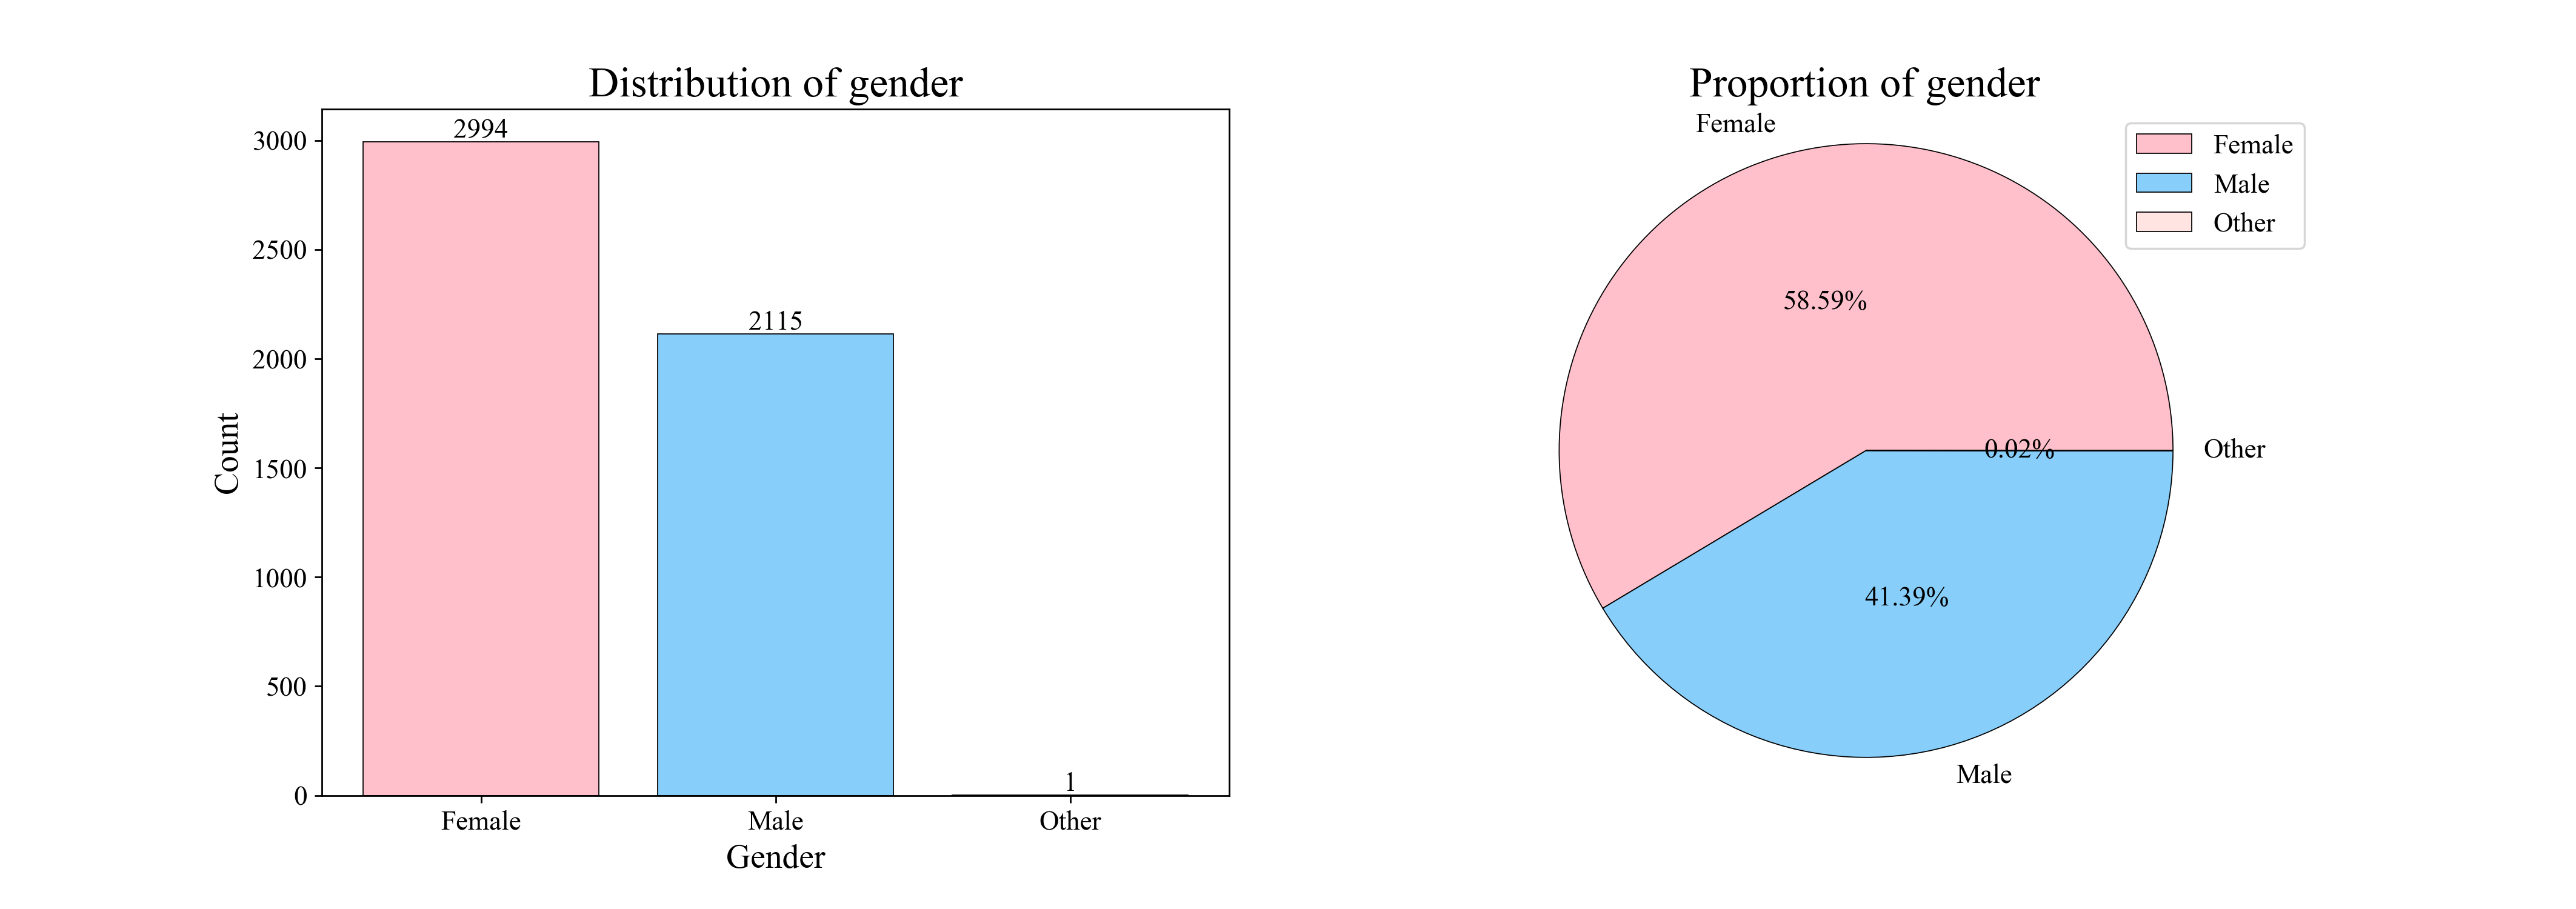
\includegraphics[width=13.5cm]{./images/gender_bar_pie.png}

\subsection{Hypertension}
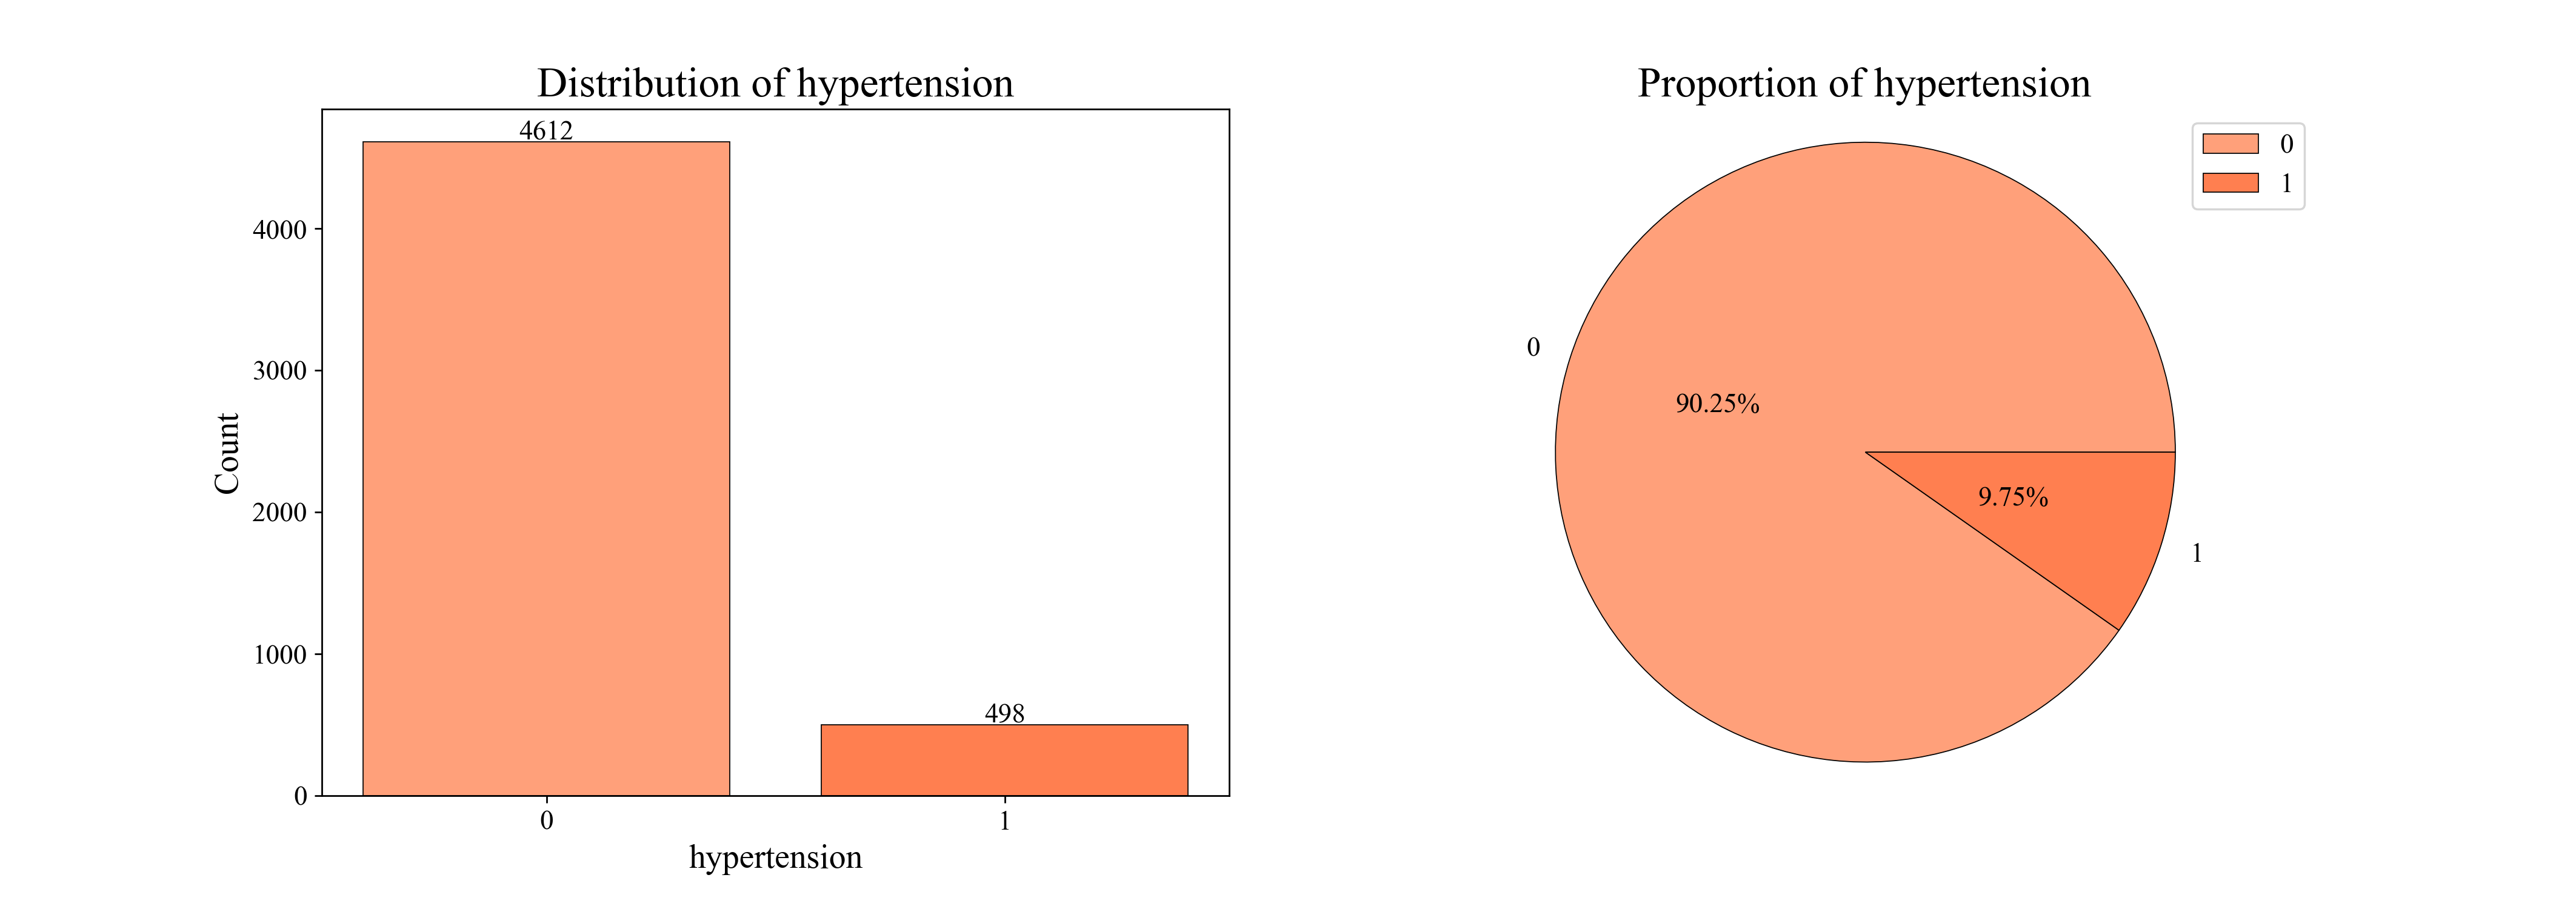
\includegraphics[width=13.5cm]{./images/hypert_bar_pie.png}

\subsection{Heart Disease}
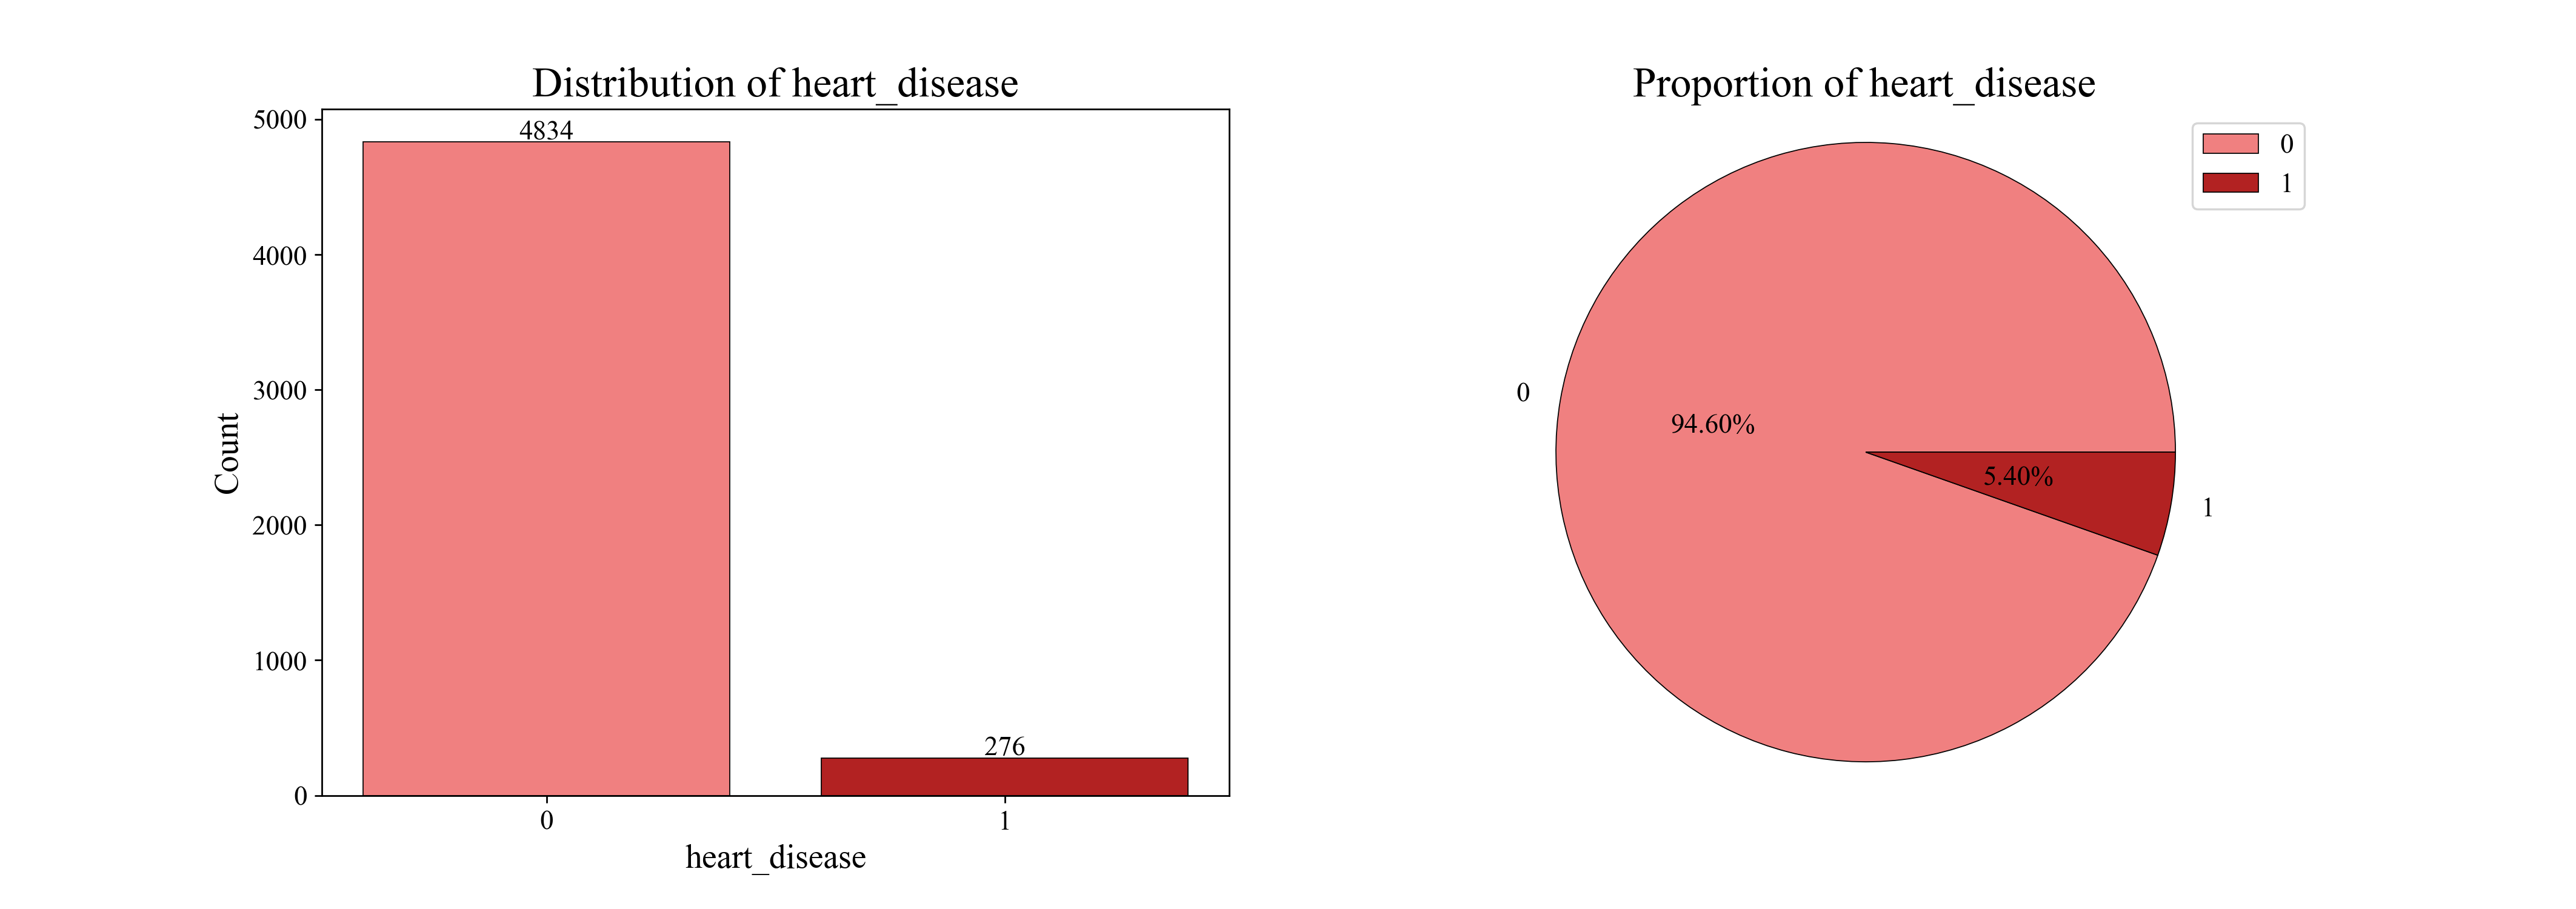
\includegraphics[width=13.5cm]{./images/heartd_bar_pie.png}

\subsection{Ever married}
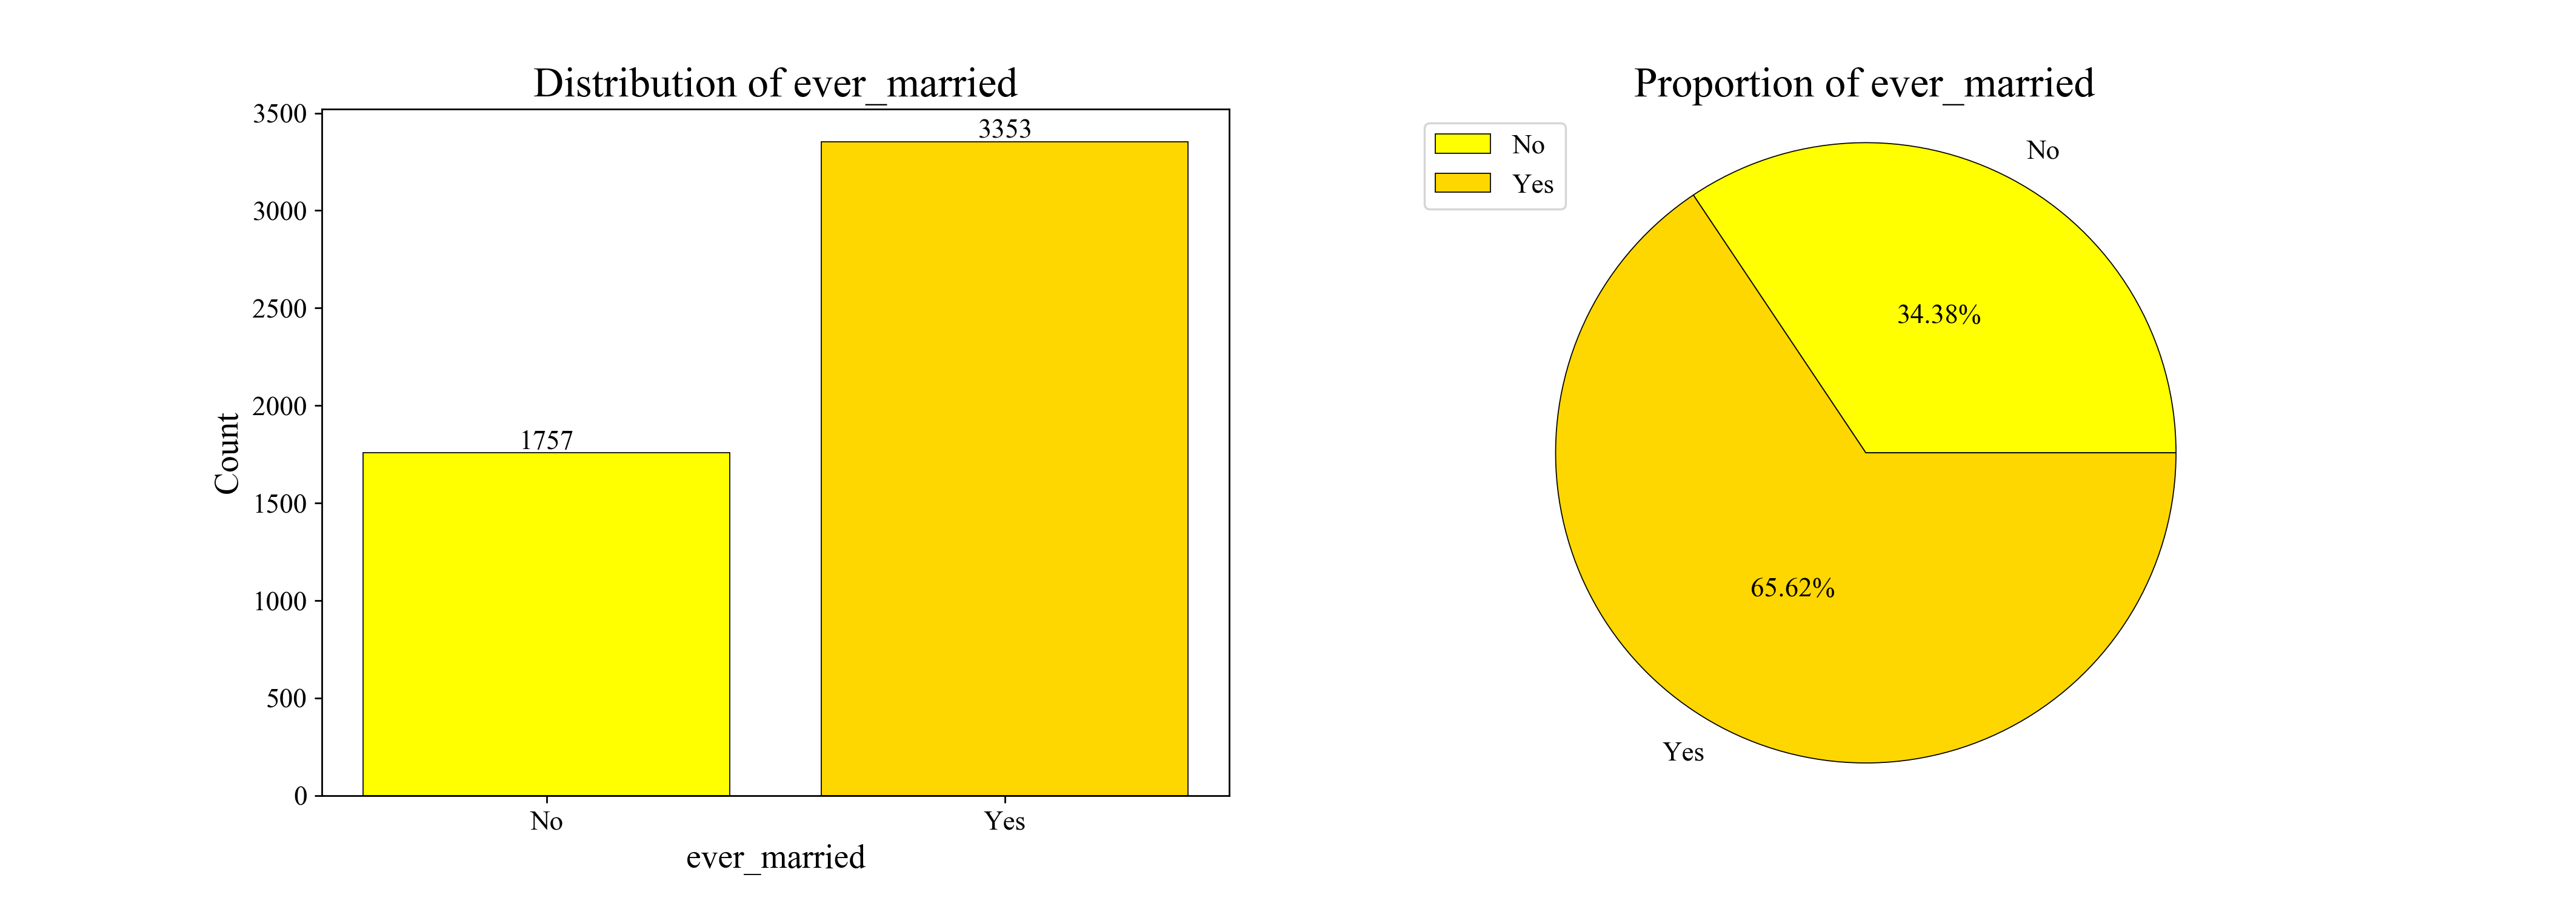
\includegraphics[width=13.5cm]{./images/evermarry_bar_pie.png}

\subsection{Residence type}
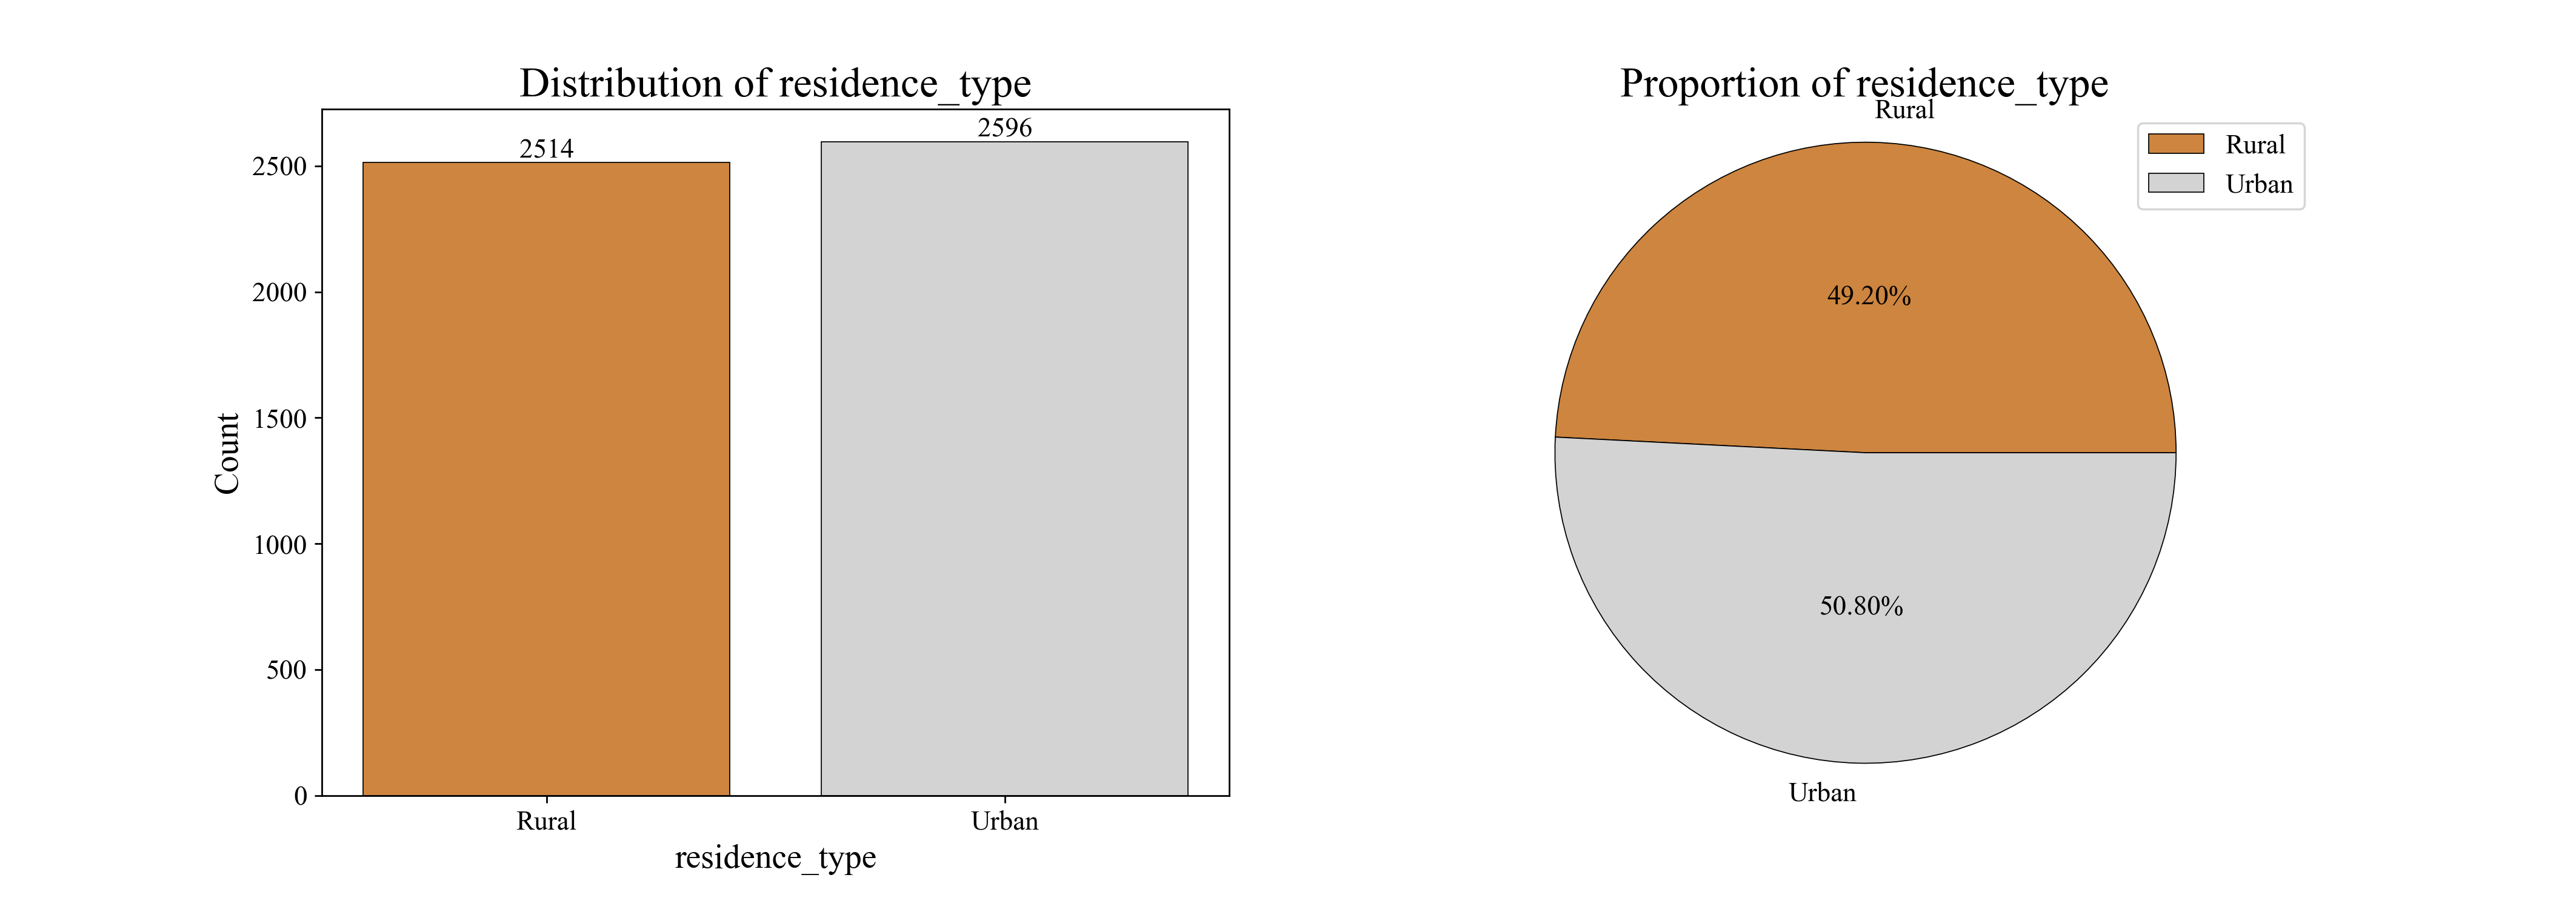
\includegraphics[width=13.5cm]{./images/resit_bar_chart.png}

\subsection{Stroke}
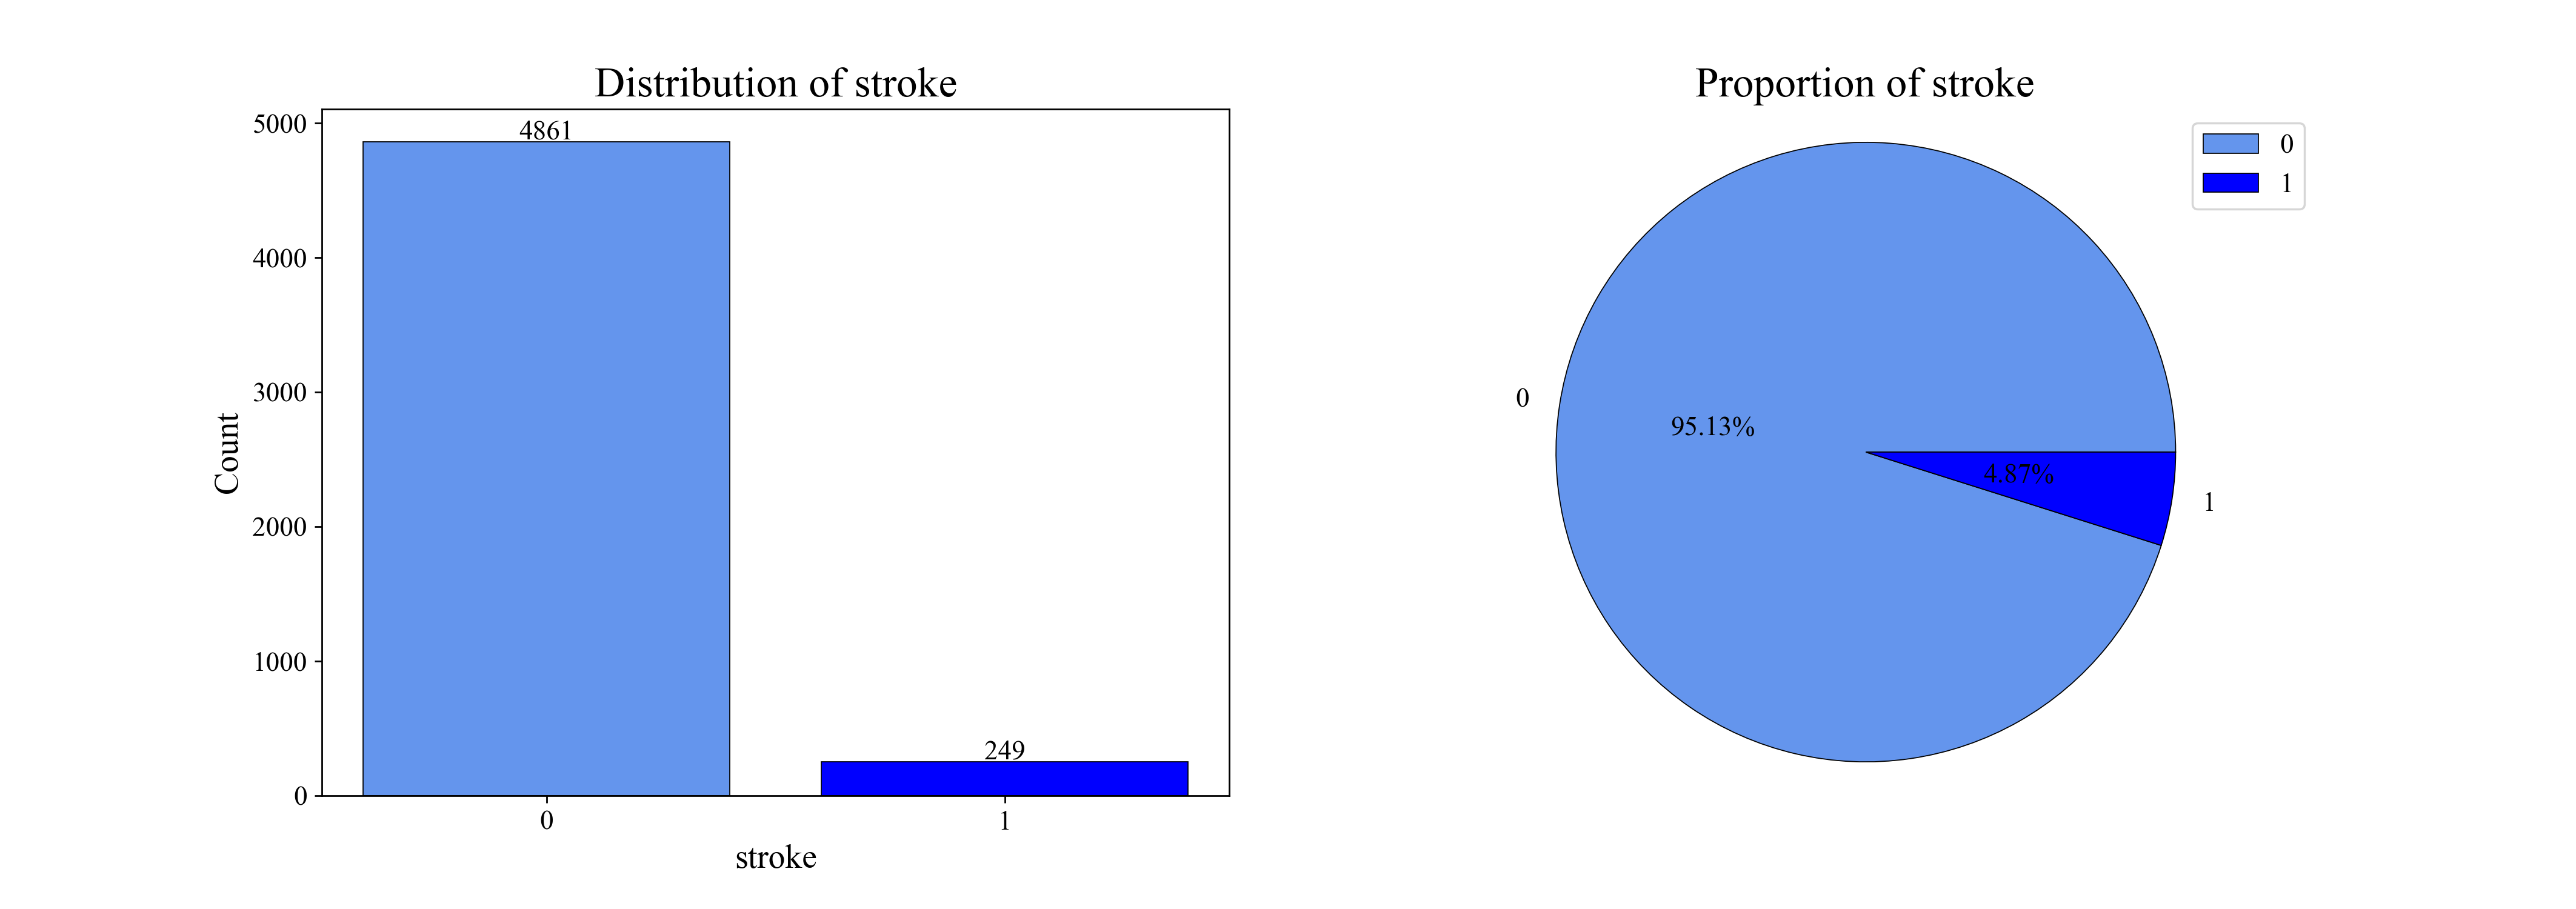
\includegraphics[width=13.5cm]{./images/stroke_bar_pie.png}

\subsection{Smoking status}
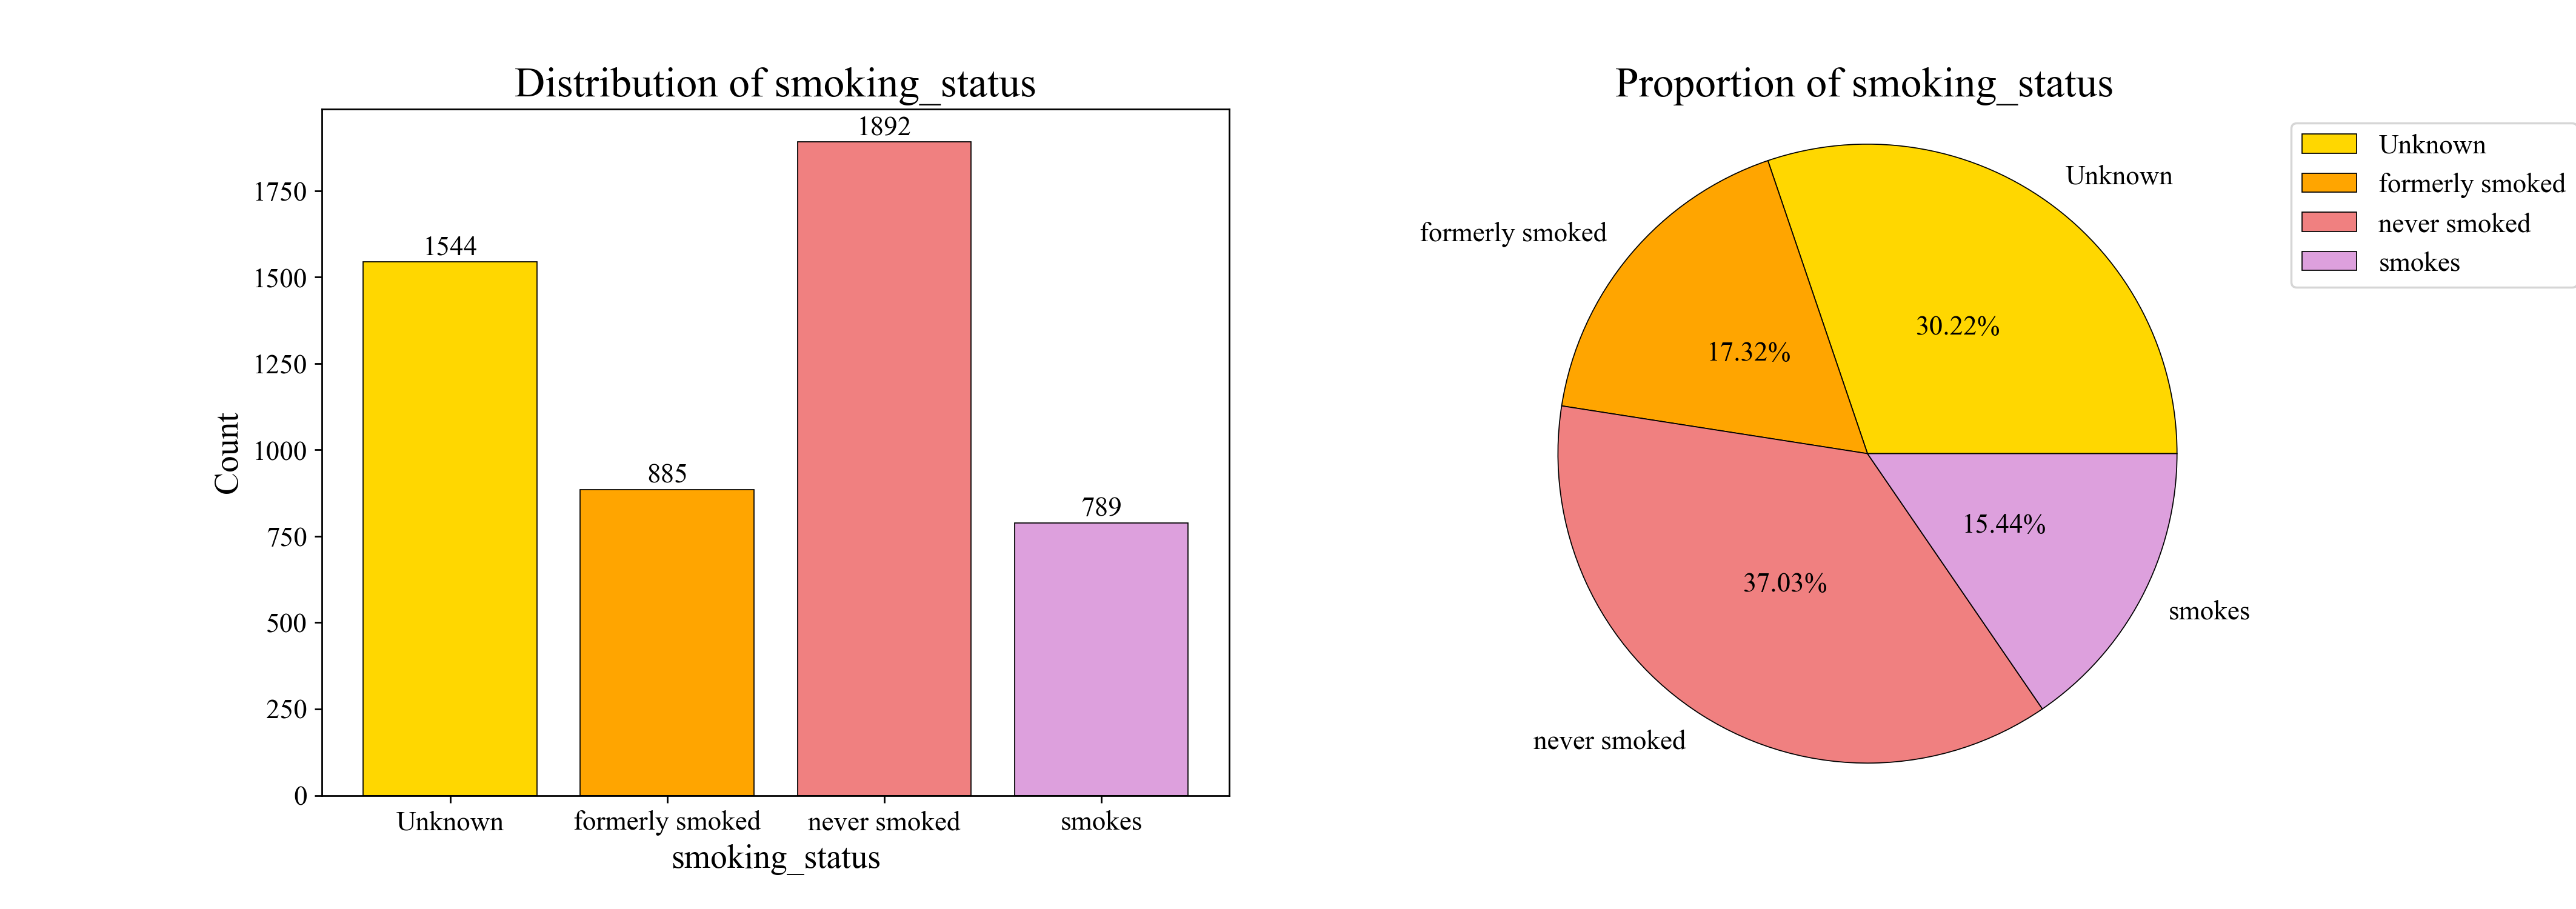
\includegraphics[width=13.5cm]{./images/smoking_bar_pie.png}

\subsection{Work type}
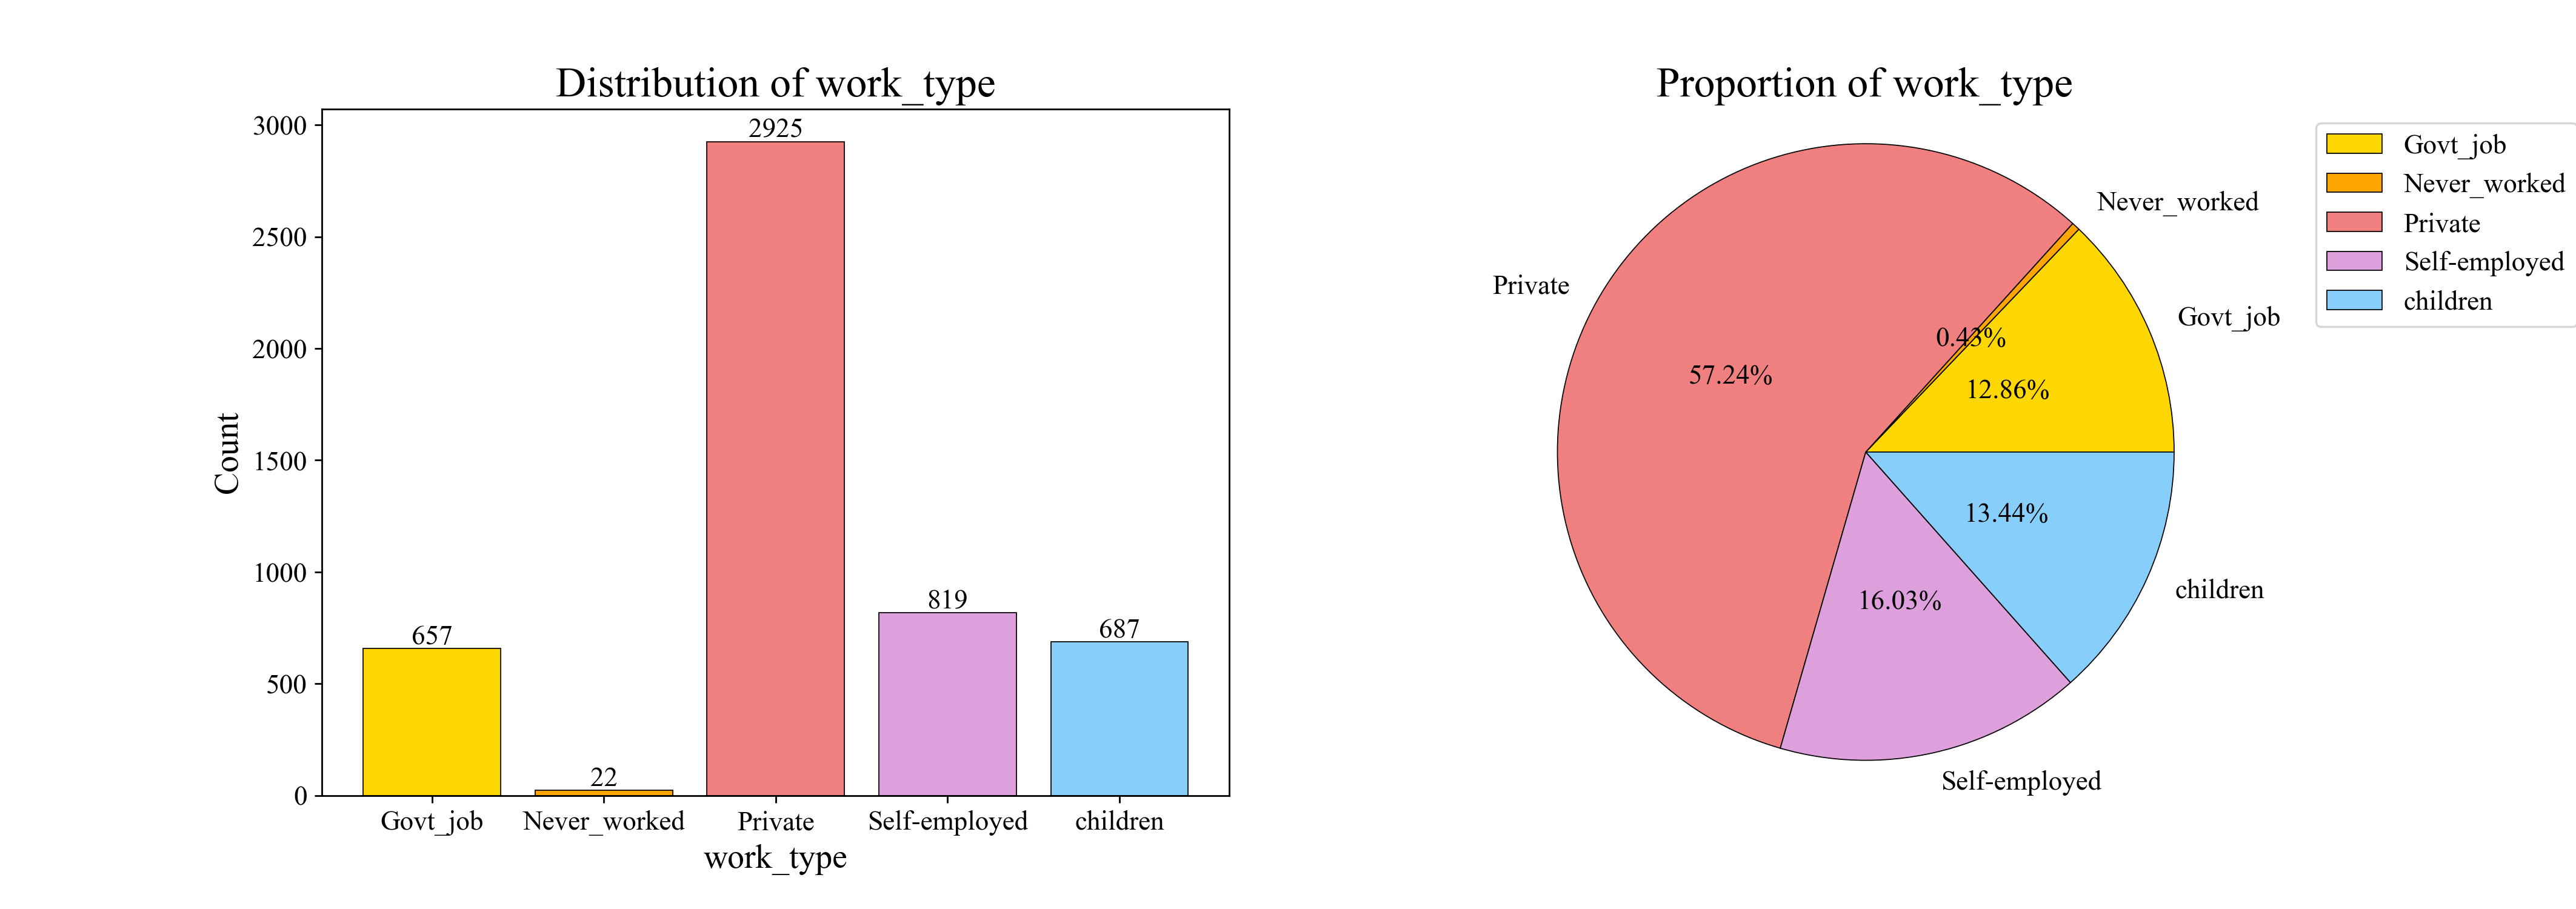
\includegraphics[width=13.5cm]{./images/worktype_bar_pie.png}

\section{單變數分析: 數值型}
\subsection{age}
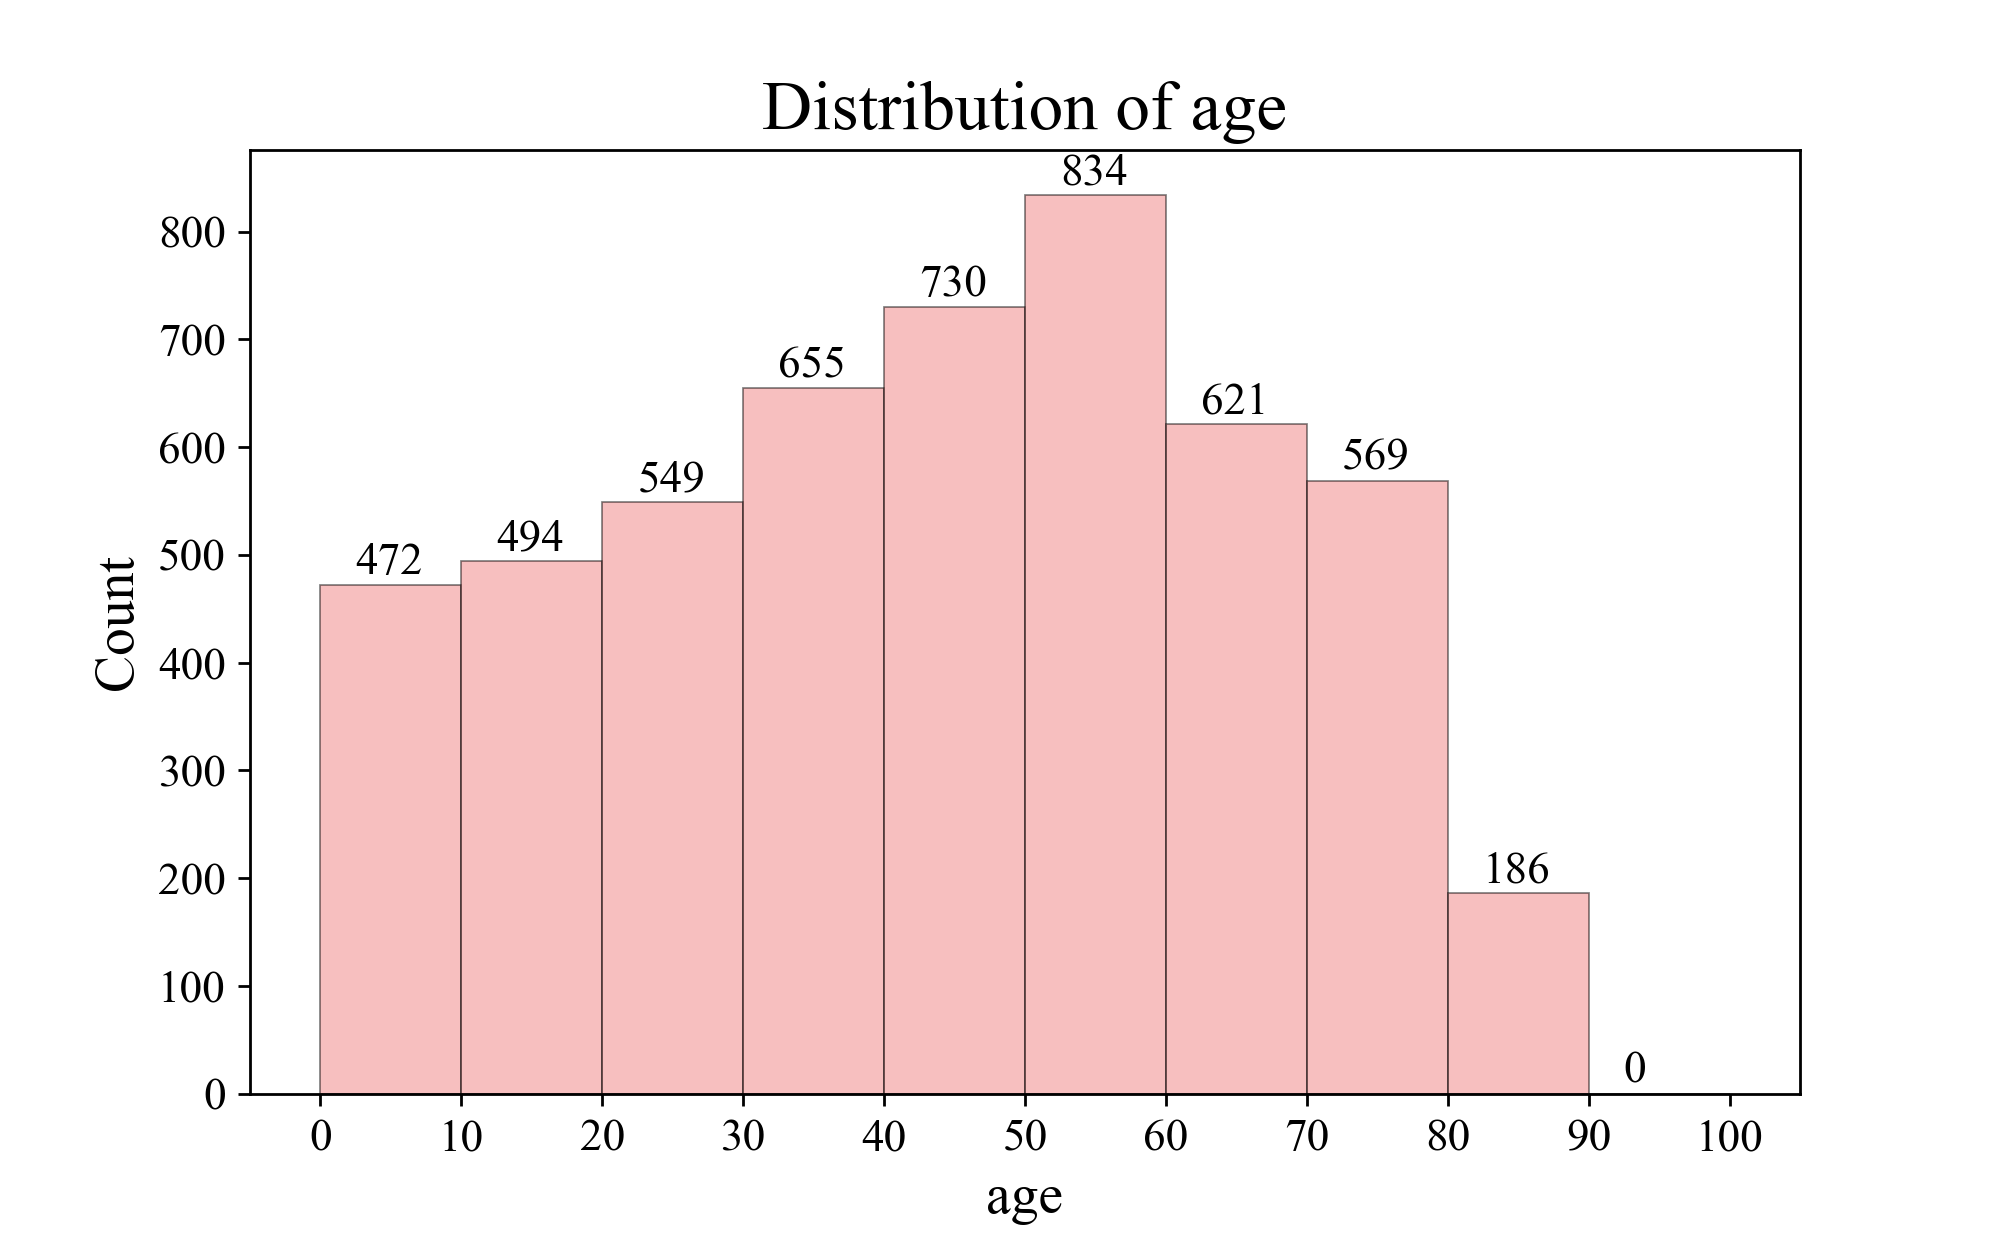
\includegraphics[height=7cm]{./images/age_distribution.png}

\subsection{Average glucose level}
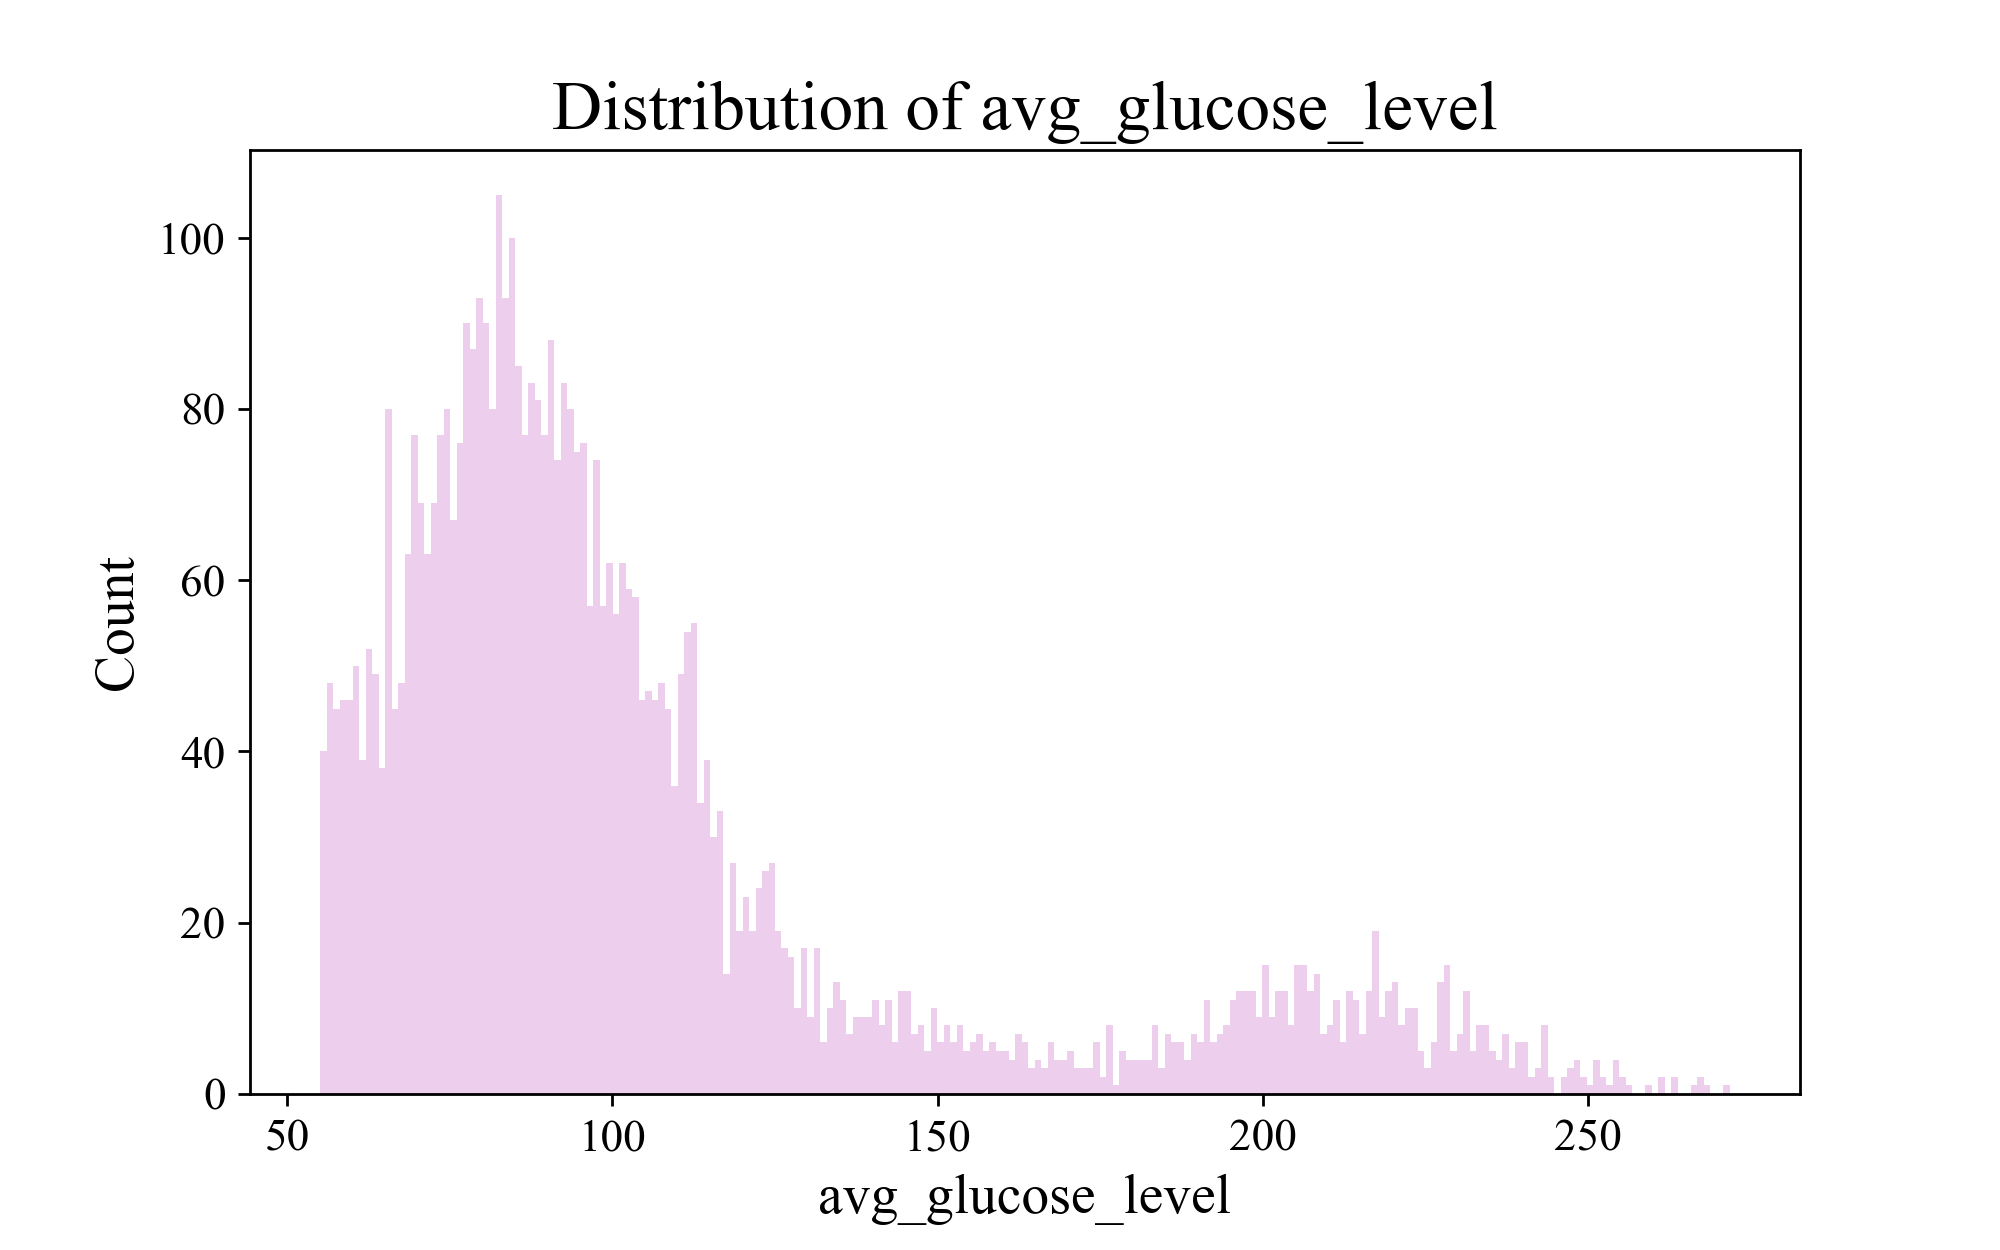
\includegraphics[height=7cm]{./images/avg_glucose_distribution.png}

\subsection{BMI}
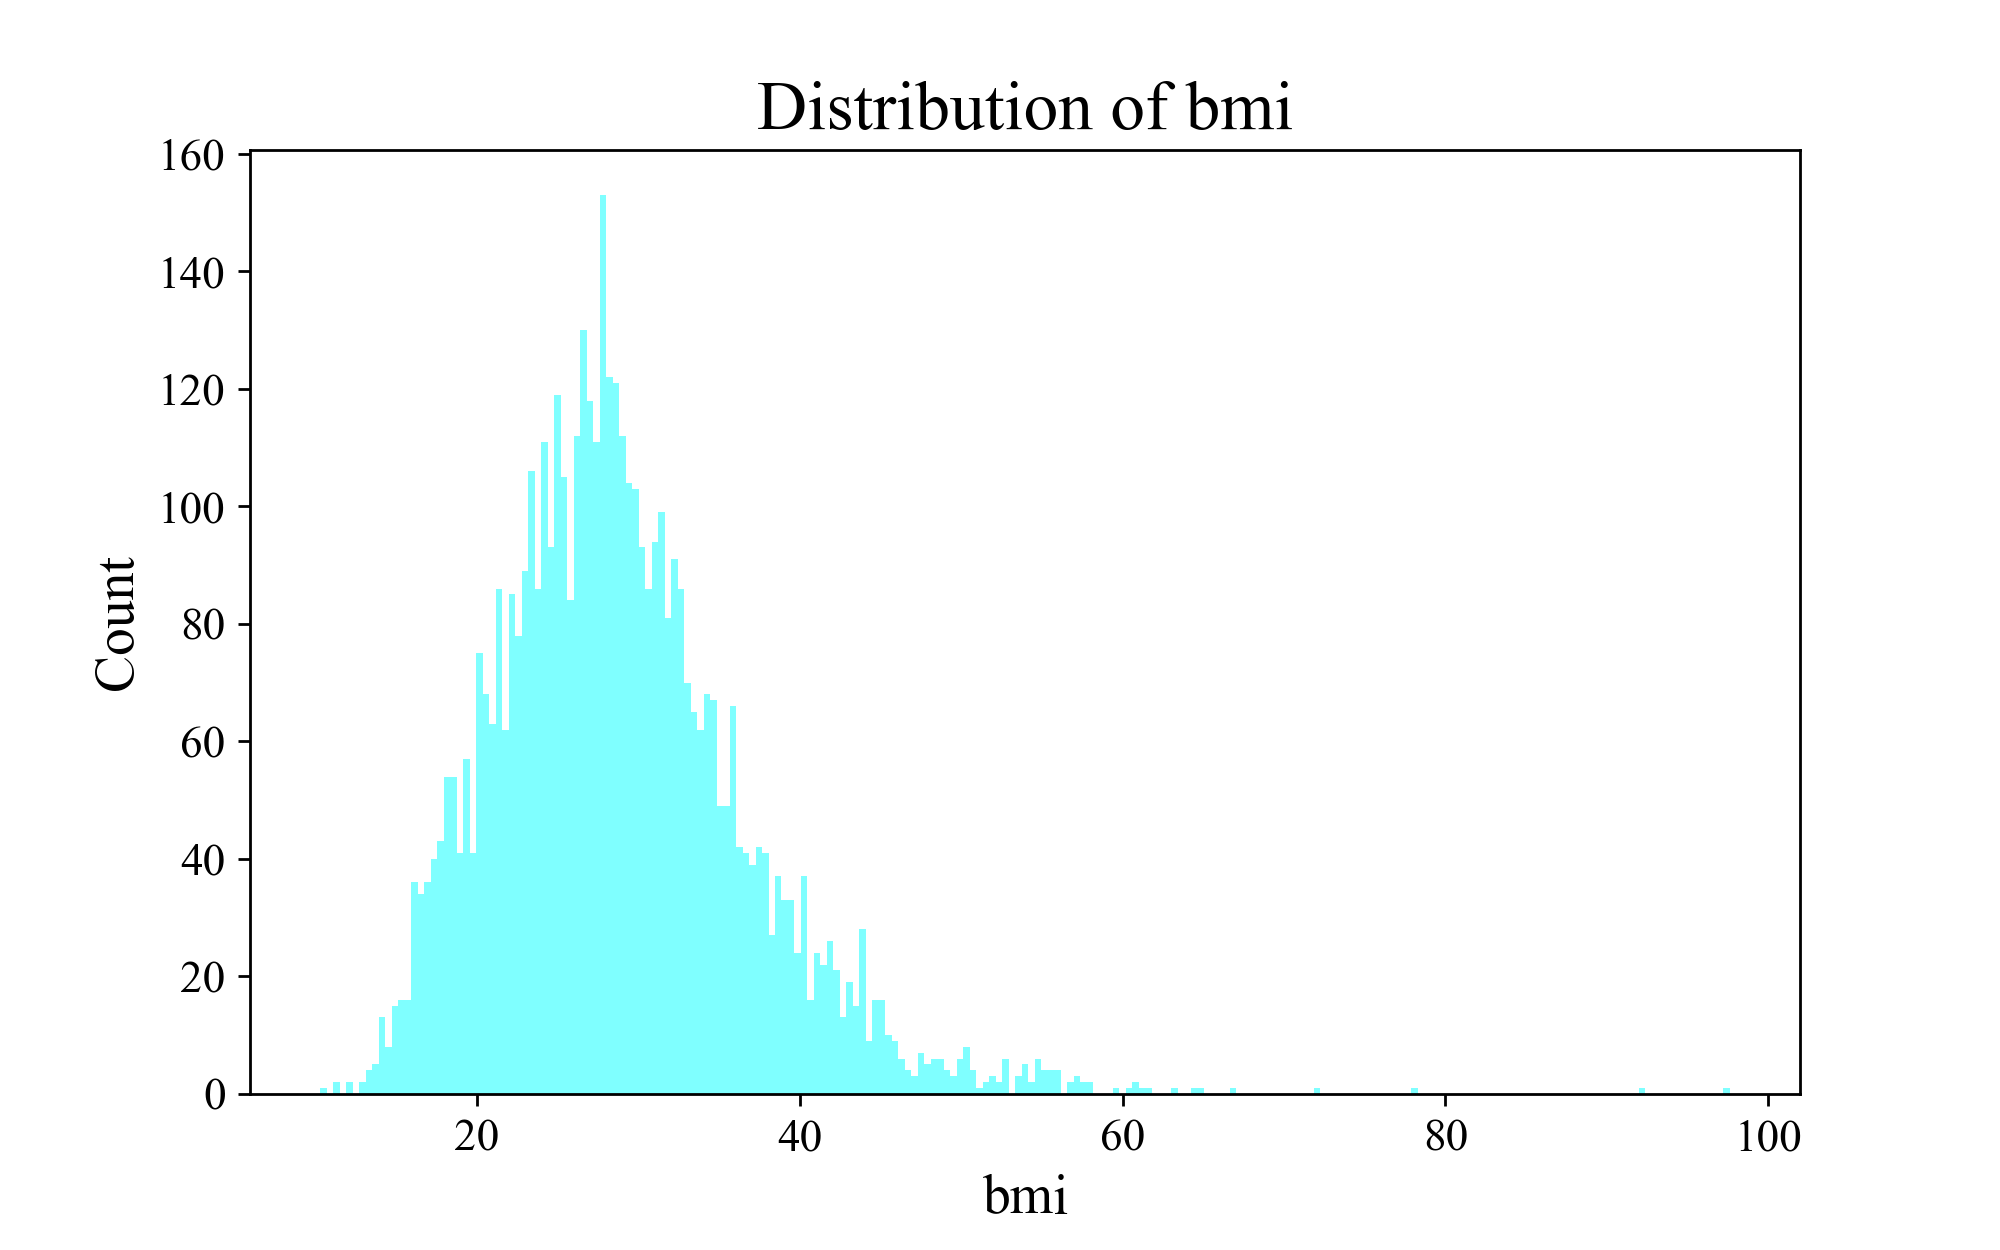
\includegraphics[height=7cm]{./images/bmi_distribution.png}




\chapter{影響中風的因素}
\section{Analysis of Contingency Table}
\subsection{中風與性別}
\begin{itemize}
    \item 基本假設:性別與中風沒有關聯
\end{itemize}
\begin{center}
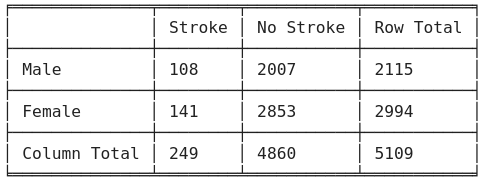
\includegraphics[width=8cm]{./two_by_two_table/gender_stroke.png}
\end{center}
\begin{itemize}
    \item 註記: 有一個性別是Other,被拿掉了
    \item Odds ratio $\hat{\theta}=1.089$
    \item 95\% Confidence Interval of $\log{(\hat{\theta})}=(-0.172, 0.342)$
    \item 結論:中風跟性別是獨立的,符合我們一開始的猜想
\end{itemize}

\subsection{中風與居住環境}
\begin{itemize}
    \item 基本假設:只有一點點關聯,鄉下的中風比例可能比住在城市的低
\end{itemize}
\begin{center}
    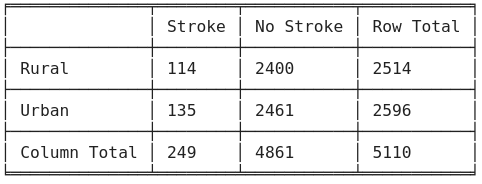
\includegraphics[width=8cm]{./two_by_two_table/resitype_stroke.png}
\end{center}
\begin{itemize}
    \item Odds ratio $\hat{\theta}=0.866$
    \item 95\% Confidence Interval of $\log{(\hat{\theta})}=(-0.400, 0.112)$
    \item 雖然資料符合我們的猜想,鄉下中風的比例比較低,但是95\%的信賴區間包含0,表示 $\log{(\hat{\theta})}$ 與0無顯著差異
    \item 結論:中風與居住環境是獨立的
\end{itemize}

\subsection{中風與婚姻}
\begin{itemize}
    \item 基本假設:婚姻與中風沒有關聯
\end{itemize}
\begin{center}
    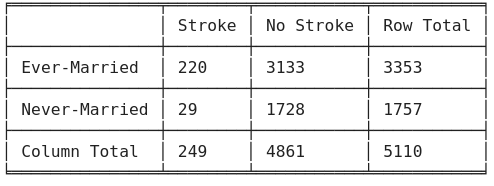
\includegraphics[width=8cm]{./two_by_two_table/evermarry_stroke.png}
\end{center}
\begin{itemize}
    \item Odds ratio $\hat{\theta}=4.184$
    \item 95\% Confidence Interval of $\log{(\hat{\theta})}=(1.040, 1.823)$
    \item 95\%的信賴區間不包含0,表示 $\log{(\hat{\theta})}$ 與0有顯著差異。
    \item 結論:跟我們的基本假設相反,中風跟"有無結過婚"有關聯
\end{itemize}
Fix column比較:
\begin{itemize}
    \item 中風患者: $\frac{\text{Ever-Married}}{\text{Never-Married}}=7.59$
    \item 非中風者: $\frac{\text{Ever-Married}}{\text{Never-Married}}=1.81$
    \item 中風患者中"結婚與沒結婚"的比例高於非中風者
\end{itemize}

\subsection{中風與壓力}
\begin{itemize}
    \item 基本假設:壓力愈大的人愈容易中風
\end{itemize}
\begin{center}
    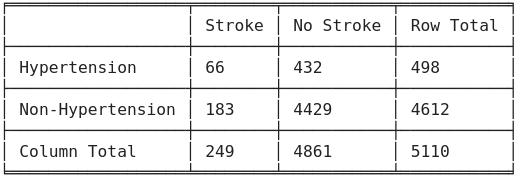
\includegraphics[width=8cm]{./two_by_two_table/hypert_stroke.png}
\end{center}
\begin{itemize}
    \item Odds ratio $\hat{\theta}=3.698$
    \item 95\% Confidence Interval of $\log{(\hat{\theta})}=(1.009, 1.606)$
    \item 95\%的信賴區間不包含0,表示 $\log{(\hat{\theta})}$ 與0有顯著差異。
    \item 結論:中風跟壓力有關聯
\end{itemize}
Fix column比較:
\begin{itemize}
    \item 中風患者: $\frac{\text{Hypertension}}{\text{Non-Hypertension}}=0.36$
    \item 非中風者: $\frac{\text{Hypertension}}{\text{Non-Hypertension}}=0.10$
    \item 符和基本假設,壓力愈大的人愈容易中風
\end{itemize}

\subsection{中風與心臟病}
\begin{itemize}
    \item 基本假設:中風是心血管疾病,要與心臟病相關
\end{itemize}
\begin{center}
    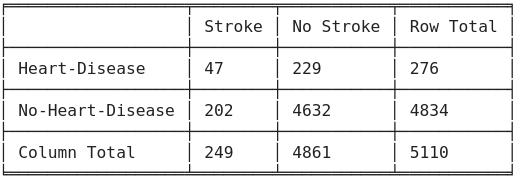
\includegraphics[width=8cm]{./two_by_two_table/heartd_stroke.png}
\end{center}
\begin{itemize}
    \item Odds ratio $\hat{\theta}=4.706$
    \item 95\% Confidence Interval of $\log{(\hat{\theta})}=(1.205, 1.893)$
    \item 95\%的信賴區間不包含0,表示 $\log{(\hat{\theta})}$ 與0有顯著差異。
    \item 結論:中風跟心臟病有關聯
\end{itemize}
Fix column比較:
\begin{itemize}
    \item 中風患者: $\frac{\text{Heart-Disease }}{\text{No-Heart-Disease}}=0.23$
    \item 非中風者: $\frac{\text{Heart-Disease }}{\text{No-Heart-Disease}}=0.05$
    \item 符和基本假設,中風患者中有心臟病的比例高
\end{itemize}

\subsection{中風與抽煙習慣}
\begin{itemize}
    \item 基本假設:有抽煙的人比較容易中風
\end{itemize}
\begin{center}
    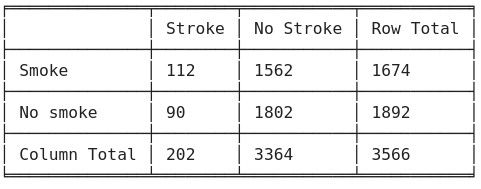
\includegraphics[width=8cm]{./two_by_two_table/smoke_stroke.png}
\end{center}
\begin{itemize}
    \item 註記: unknown有1544個資料點,被拿掉了
    \item 註記: smoke包含smokes與formerly smoked
    \item Odds ratio $\hat{\theta}=1.436$
    \item 95\% Confidence Interval of $\log{(\hat{\theta})}=(0.076, 0.647)$
    \item 95\%的信賴區間不包含0,表示 $\log{(\hat{\theta})}$ 與0有顯著差異。
    \item 結論:中風跟抽煙有關聯。但相比於婚姻、壓力與心臟病,抽煙的$\hat{\theta}$比較靠近$1$,表示抽煙相對來說不是一個重要的因子
\end{itemize}
Fix column比較:
\begin{itemize}
    \item 中風患者: $\frac{\text{Smoke}}{\text{No smoke}}=1.24$
    \item 非中風者: $\frac{\text{Smoke}}{\text{No smoke}}=0.87$
    \item 符和基本假設,中風患者中有抽煙的比例高
\end{itemize}

\subsection{中風與年齡}
\begin{center}
    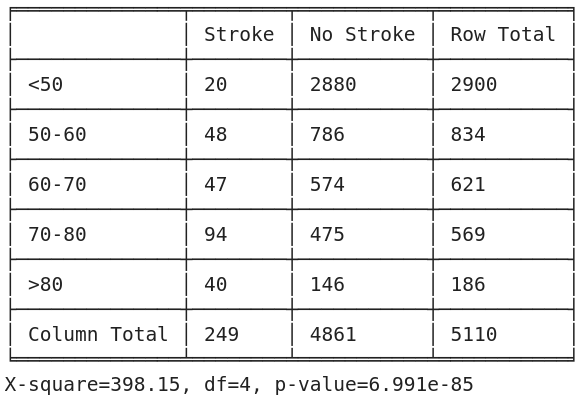
\includegraphics[width=8cm]{./chisquare/age_stroke.png}
\end{center}

\subsection{中風與血糖}
分類依據:
\begin{center}
    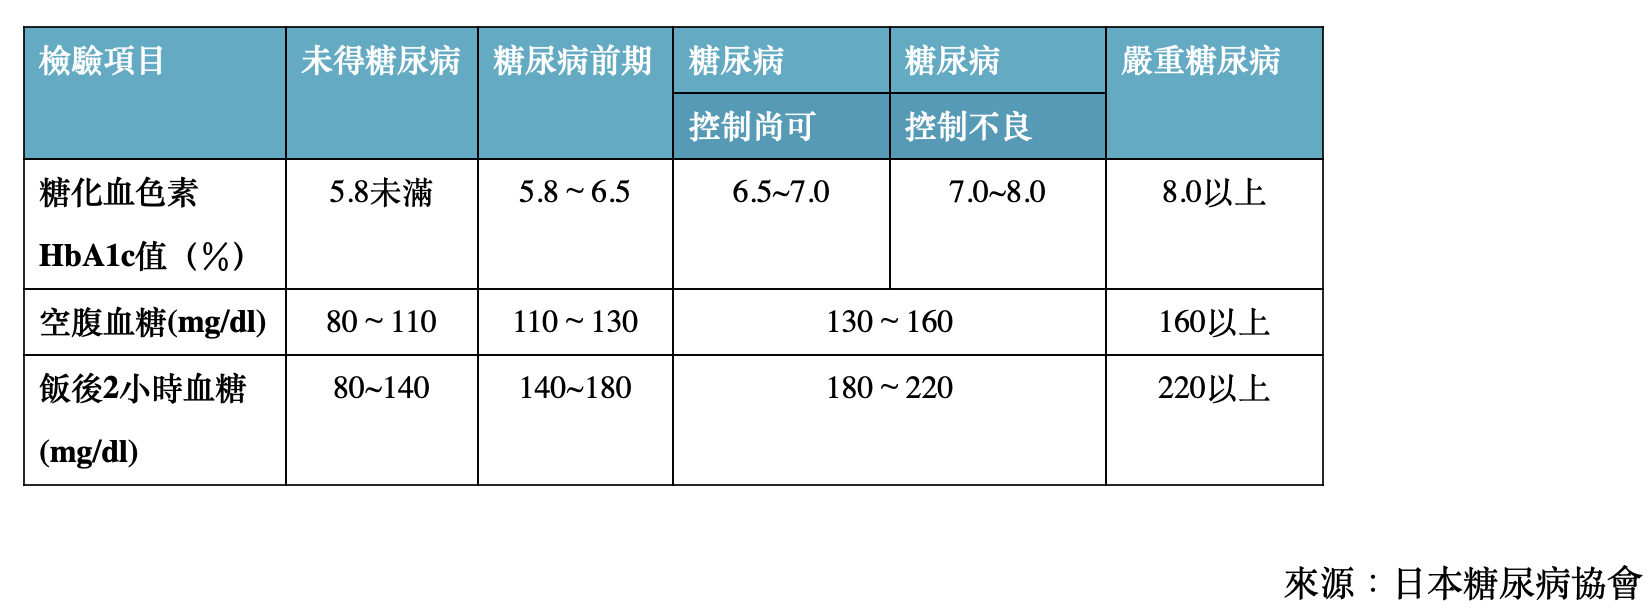
\includegraphics[width=8cm]{./images/glucose_category_ref.png}
\end{center}
$\chi^2$ test:
\begin{center}
    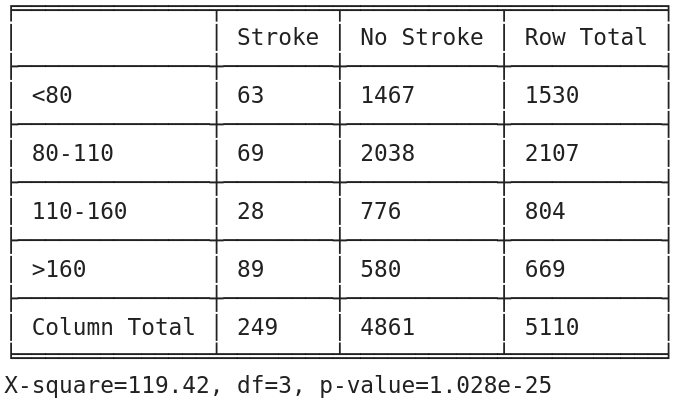
\includegraphics[width=8cm]{./chisquare/glucose_stroke.png}
\end{center}

\subsection{中風與BMI}
分類依據:
\begin{center}
    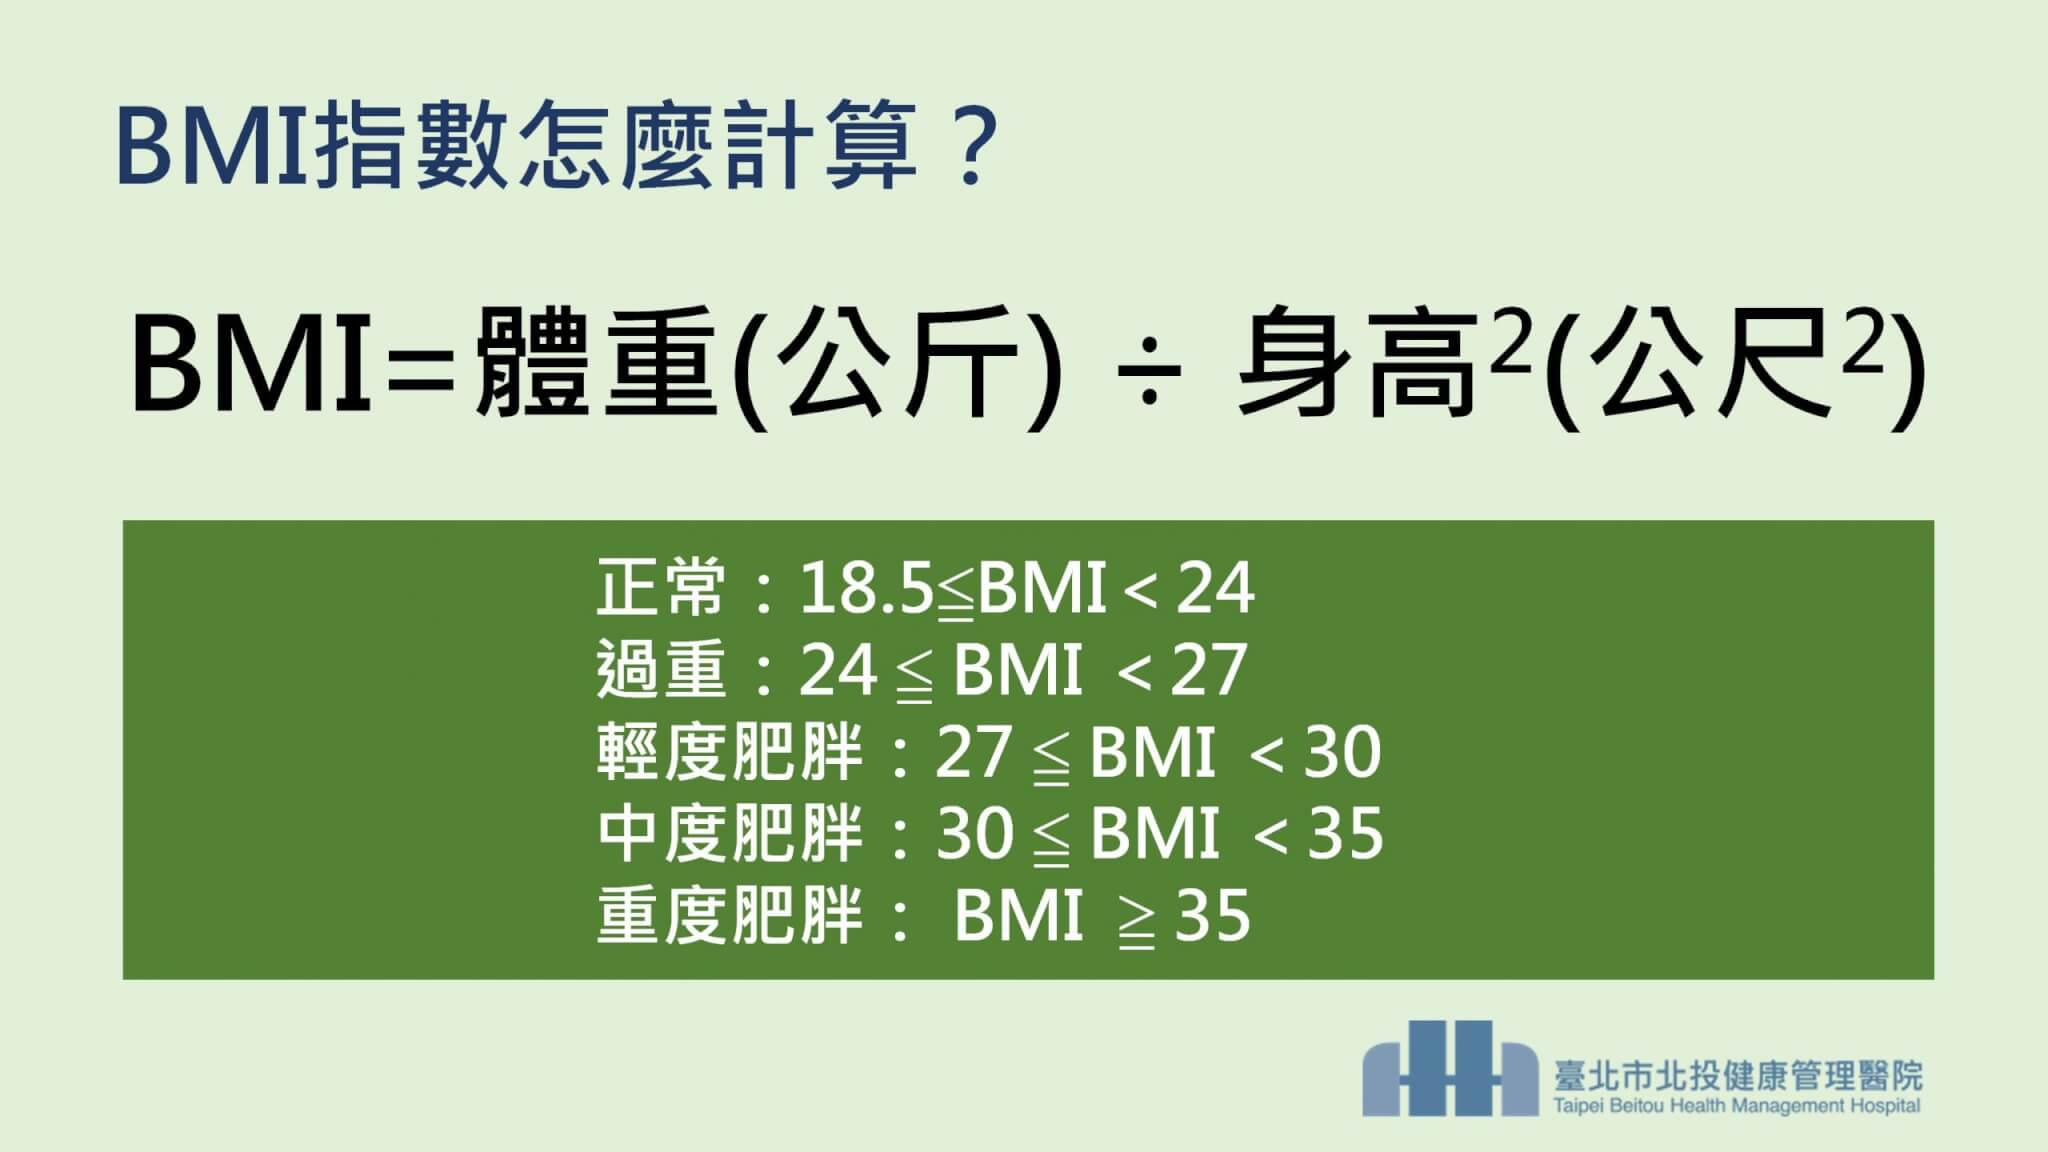
\includegraphics[width=8cm]{./images/bmi_category_ref.jpg}
\end{center}
$\chi^2$ test:
\begin{center}
    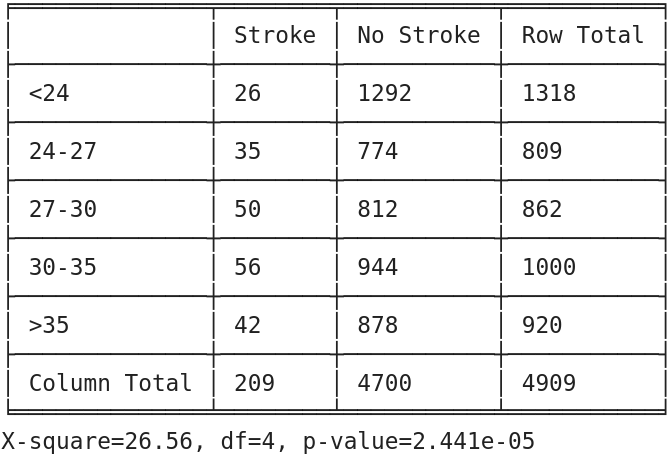
\includegraphics[width=8cm]{./chisquare/bmi_stroke.png}
\end{center}



%-------------------------------------------------------------------------------
%	BIBLIOGRAPHY
%-------------------------------------------------------------------------------
\addtocontents{toc}{\vspace{2em}} % Add a gap in the Contents, for aesthetics
\bibliographystyle{pnas-new}
\bibliography{reference} % The references information are stored in the file named "Thesis_bibliography.bib"

\end{CJK*}
\end{document}